\documentclass{article}
\usepackage{tikz}
\usetikzlibrary{shapes.geometric}

\begin{document}

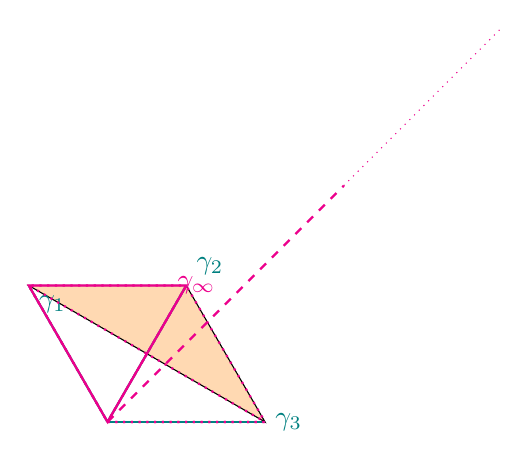
\begin{tikzpicture}[scale=2]
    % Define coordinates
    \coordinate (O) at (0,0);
    \coordinate (A) at (1,0);
    \coordinate (B) at (0.5,0.866);
    \coordinate (C) at (-0.5,0.866);
    
    % Draw the convex hull (orange filled shape)
    \draw[fill=orange!30] (A) -- (B) -- (C) -- cycle;
    
    % Draw the coupling vectors (teal vectors)
    \draw[teal, thick] (O) -- (A) node[right] {$\gamma_3$};
    \draw[teal, thick] (O) -- (B) node[above right] {$\gamma_2$};
    \draw[teal, thick] (O) -- (C) node[below right] {$\gamma_1$};
    
    % Draw the distance vector (purple vector)
    \draw[magenta, dashed, thick] (O) -- (1.5,1.5) node[midway, above left] {$\gamma_\infty$};
    
    % Draw the dotted line for the asymptotic behavior
    \draw[dotted, magenta] (1.5,1.5) -- (2.5,2.5);
    
    % Draw the triangle (for reference)
    \draw[magenta, thick] (O) -- (B) -- (C) -- cycle;
    
    % Draw the triangle edges
    \draw[magenta, thick, dotted] (O) -- (A) -- (B) -- cycle;
    \draw[magenta, thick, dotted] (O) -- (A) -- (C) -- cycle;
    \draw[magenta, thick, dotted] (O) -- (B) -- (C) -- cycle;
\end{tikzpicture}

\end{document}